%%%%%%%%%%%%%%%%%%%%%%%%%%%%%%%%%%%%%%%%%%%%%%%%%%%
% DOCUMENT CLASS DECLARATION
%%%%%%%%%%%%%%%%%%%%%%%%%%%%%%%%%%%%%%%%%%%%%%%%%%%
%% Use the following options:
% \documentclass[paper type% ("letterpaper" required)
% , one or two sided% ("oneside" or "twoside")%
% , font size% ("12pt" required)%
% , document type% ("these", "memoire", "memoireprojet" or "thesepararticles")%
% , document language ("francais" or "english)%
% , addition options% ("creativecommons" if the document is under the creative commons license, "hyperref", "withAlgo2e" to use algorithm2e package with proper formating)
%]{thETS}

%% Exemple with a Ph.D thesis under creative commons, using hyperref
\documentclass[letterpaper%
, twoside%
, 12pt%
,these%
, english%
,creativecommons,hyperref, withAlgo2e %
]{thETS}

%%%%%%%%%%%%%%%%%%%%%%%%%%%%%%%%%%%%%%%%%%%%%%%%%%%
% IMPORTANT: PRINTING WITH THE PROPER MARGINS
%%%%%%%%%%%%%%%%%%%%%%%%%%%%%%%%%%%%%%%%%%%%%%%%%%%
%% If you create a pdf with pdftex, and print it using acrobat reader, set the
%% "scaling" option to "none" to print with the proper margins.
%%%%%%%%%%%%%%%%%%%%%%%%%%%%%%%%%%%%%%%%%%%%%%%%%%%
\usepackage{comment}
\usepackage[toc,page]{appendix}
\usepackage{graphicx}
\usepackage{color}
 \usepackage[table,xcdraw]{xcolor}
\usepackage{pdfpages} 
\usepackage{pgfgantt}
\usepackage{xcolor}


%%%%%%%%%%%%%%%%%%%%%%%%%%%%%%%%%%%%%%%%%%%%%%%%%%%
% DECLARATION OF AN ADDITION LIST OF REFERENCES
%%%%%%%%%%%%%%%%%%%%%%%%%%%%%%%%%%%%%%%%%%%%%%%%%%%
%% Exemple of an additional list of references called "refs"
% "refs" is used as a suffix to all bibliography related commands
\newcites{refs}{LIST OF REFERENCES}

%%%%%%%%%%%%%%%%%%%%%%%%%%%%%%%%%%%%%%%%%%%%%%%%%%%
% TITLE PAGE OPTIONS
%%%%%%%%%%%%%%%%%%%%%%%%%%%%%%%%%%%%%%%%%%%%%%%%%%%

\title{MediatorBot: An intelligent conversational bot of supporting students working together in a collaborative E-learning platform by using a Intelligent Tutor System}

\author{Vu Do Dung}
%\authorcopyright{First name Last name}

\datesoutenance{"20th, April, 2019"}

\datedepot{"20th, March, 2019"}

\directeur{Prof. }{Sylvie Ratt\'e}{Département de génie logiciel et des TI
}

%\directeur{Mrs.}{Prénom Nom}{Nom du département et institution}

\codirecteur{Mrs.}{First Name Last Name}{Department and institution}

%\codirecteurB{M.}{Prénom Nom}{département et institution}

\president{M.}{First Name Last Name}{Department and institution}

\examinexterne{M.}{First Name Last Name}{Department and institution}

%\jury{Mme.}{Prénom Nom}{département et institution}{}

%%%%%%%%%%%%%%%%%%%%%%%%%%%%%%%%%%%%%%%%%%%%%%%%%%%
% CHANGING THE NAME OF THE DIPLOMA
%%%%%%%%%%%%%%%%%%%%%%%%%%%%%%%%%%%%%%%%%%%%%%%%%%%
%% It is possible to change the name of the diploma by redefining
% the command \lediplome, as follows:
%\renewcommand{\lediplome}{OF A MASTER’S DEGREE\\WITH THESIS IN ELECTRICAL ENGINEERING\\M.A.Sc.}

\listfiles

%%%%%%%%%%%%%%%%%%%%%%%%%%%%%%%%%%%%%%%%%%%%%%%%%%%
% ACTUAL DOCUMENT
%%%%%%%%%%%%%%%%%%%%%%%%%%%%%%%%%%%%%%%%%%%%%%%%%%%
\usepackage{xcolor}
%\definecolor{light-gray}{gray}{0.95}
%\newcommand{\code}[1]{\colorbox{light-gray}{\texttt{#1}}}
\newcommand{\code}[1]{{\texttt{#1}}}
\begin{document}

\pagenumbering{Roman}

%%- Title page -%%
%\maketitle 


%%- Jury presentation -%%
\presentjury
\begin{comment}
%%- Foreword -%%
\begin{foreword}

%\lipsum[1] % Texte de remplissage pour donner un exemple de la mise en page

\end{foreword}

\end{comment}
\begin{comment}
%%- Acknowledgements -%%
\begin{acknowledgements}

%\lipsum[1] % Text filling, to have an example of the layout


\end{acknowledgements}
\end{comment}

%%- Summary -%%
\begin{comment}
\begin{summary}{French title}{mot-clé1, mot-clé2}

%\lipsum[1] % Text filling, to have an example of the layout

\end{summary}
\end{comment}

%%- Abstract -%%
\begin{abstract}{Intelligent Tutor, Artificial Intelligence, Natural Language Processing}

%\lipsum[1] % Text filling, to have an example of the layout

The interactivity of online learning is very important through it becomes popular. Moreover, the usage of Artificial Intelligence application is growing accelerated in modern years and in many sectors. In order to improve the interactivity and effectiveness of E-Learning environment in supporting students collaborate together, a conversational bot called MediatorBot is considered. As a part of Artificial Intelligence application, it generates hints to help users solve their obscure problem according to the given lecture or assignment. It can be integrated with an Intelligent Tutor System (ITS) as an add-in. MediatorBot contains the knowledge of a given specific domain (e.g., deep learning) which is valuable to deliver an appropriate answer to the users' questions. Especially, it monitors the conversations of each student groups, identifies the debated or clarified problem, and the opportunities for intervention. In the original ITS, the bot answers the question or inquiry of the user. In this research, the authors would like to overcome the ITS by improving its knowledge, determining intervention opportunities according to the group conversation within a given domain-specific online curriculum. As to encourage students knowledge approach, several features are being examined such as definition extractor, hints generator, intervention investigator, etc., This will allow the student to directly follow the maintenance of a specific topic and build their knowledge in an effective way. In addition, an enhancement to engage all the students following the conversation is proposed to help them come up with the lecture. With this enhancement, MediatorBot can give a recommendation of solutions for users to ask. All of the functions are measured using the users' experiment feedback in parallel with the experts' evaluation.
\end{abstract}


%%- Table of contents -%%
\tableofcontents


%%- List of tables -%%
\listoftables


%%- List of figures -%%
\listoffigures

%\listofalgorithms


%%- List of abbreviations -%%
\begin{listofabbr}[3cm]
\item [AI] Artificial Intelligence
\item [ITS] Intelligent Tutoring Systems
\item [CSCL]  Computer-Supported Collaborative Learning
\item [RNN] Recurrent Neural Network 
\item [MLE] Maximum Likelihood Estimation
\item [NLP] Natural Language Processing
\item [SVM] Support Vector Machine
\item [CNNs] Convolution Neural Networkss

\end{listofabbr}


%%- List of symbols -%%
%\begin{listofsymbols}[3cm]


%\end{listofsymbols}


\cleardoublepage

\pagenumbering{arabic}

% Marginpar to the left of the document
\reversemarginpar

%%%%%%%%%%%%%%%%%%%%%%%%%%%%%%%%%%%%%%%%%%%%%%%%%%%
% THESIS EXAMPLE
%%%%%%%%%%%%%%%%%%%%%%%%%%%%%%%%%%%%%%%%%%%%%%%%%%%

\begin{introduction}

%\lipsum[1] % Text filling, to have an example of the layout

Intelligent Tutoring Systems (ITS) is developed in the early 1970s \cite{Brown}. One of the intentions in AI technologies is to create educational agents that can be adapted to the student. Because an ITS can perform various roles such as "knowledge presentation mechanisms", "knowledge processing tools", "communication tools" \cite{Tchounikine}, it succeeds through each of these functions in exciting training and cognitive development of the learner: 
\begin{itemize}
	\item     "Knowledge presentation mechanisms": By using these tools, information enhances more accessible, more up-to-date, and can be presented in various formats. It is a great stimulant for the learner's imagination, memorization, and comprehension.
	\item     "Knowledge processing tools": These tools allowance for supervision of the student better, more personalized, and adaptive learning. The learner can do their self-evaluations, get recommendations, and feedback faster.
	\item "Communication tools": These tools are utilized for projects which have human and machine communication through intelligent agents. The better communication is, the better the teaching will be and hence the more effortful learning is. 
\end{itemize}

According to the timeline of AutoTutor systems or Intelligent Tutor systems development in Figure \ref{fig:timeline}, most of them have the mission "helped students explain good answers" rather than "recognizing and correcting misconceptions" such as:
\begin{itemize}
	\item Help students construct expressions of material as answers to questions and solutions to challenging problems
	\item Ask questions that tap deep levels of reasoning and that involve collaboration
	\item Solve problems that involve deep argumentation
\end{itemize}


\begin{figure}
	\centering
	
	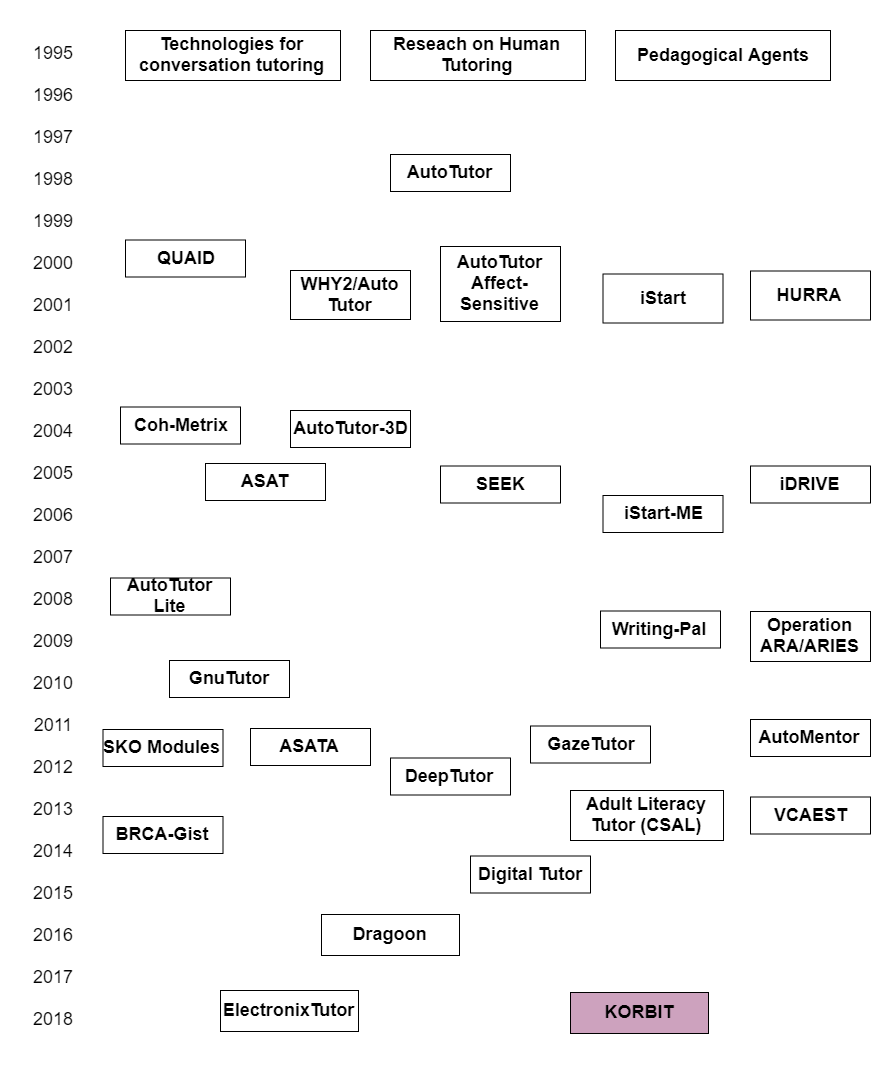
\includegraphics[width=0.75\textwidth]{Figures/ht1s.png}
	
	\caption{The time life of Intelligent Tutor System (ITS) }
	\label{fig:timeline}
\end{figure}

Conventional training or tutoring systems adapt to individual students, but they do so a level with limited options (e.g., two to five) at
each point in the student intercommunication as following:
\begin{itemize}
	\item  (a) the student  studies material presented in a
	lesson,
	\item (b) is tested with a multiple-choice test or another objective test with a small number of options,
	\item (c)
	receives feedback on the test performance,
	\item (d) re-studies,
	\item (e) progresses to a new topic if the performance in “c” exceeds the specified threshold
\end{itemize}   
An ITS monitors the detail of students' knowledge, skills, and other psychological
characteristics  and response to the student by applying computational
algorithms in artificial intelligence and cognitive science \cite{Woolf2009}\cite{Sottilare}\cite{VanLehn2006}.
For an ITS, adaptivity is so fine-grained that most of the tutorial interactions on a given topic follow the unique sequence.
ITSs have been developed for a wide range of Science, technology, engineering, and mathematics (STEM)
subject matters. Many have targeted to mathematics and
other well-formed, quantitatively precise topics. For example, there are the
Cognitive Tutors \cite{Aleven2009}\cite{Koedinger1997}\cite{Ritter2007}  and ALEKS \cite{Falmagne2013} were worked on the
areas of algebra and geometry; one assessment compared these two systems on
learning gains and resulted in a virtual tie \cite{Sabo2013}. In the area of technology and engineering, there
are ITSs on electronics \cite{Lesgold1992}\cite{Dzikovska2014}, digital information
technology \cite{Fletcher2012},
and database retrieval \cite{Mitrovic2007}.  VanLehn and his colleagues have developed Andes \cite{VanLehn2011} which was the ITS of physics.
Some ITSs concentrate on knowledge specific-domains that have a
stronger verbal foundation as opposed to mathematics
and precise analytical reasoning \cite{Johnson2016}. AutoTutor and its progenies \cite{Graesser2016}\cite{Nye2014a}\cite{Nye2014b}) help students learn by holding a conversation in natural language. Conversational agents (also known as interactive agents and
pedagogical agents) are a general class of learning environments that are intelligently adaptive \cite{Atkinson2002}\cite{Craig2002}\cite{Johnson2000}\cite{McNara2010}\cite{Moreno2001}. Conversational agents have talking heads that
speak, point, gesture, and exhibit facial expressions.
They can guide the interaction with the learner, instruct
the learner what to do, and interact with other agents to
model ideal behavior, strategies, reflections, and social
interactions \cite{Craig2015}\cite{Graesser2014}\cite{Johnson2016}\cite{Kim2007}. These agents
have been designed to represent different human instructional roles, such as experts \cite{Johnson2000}\cite{Kim2016}, tutors \cite{Nye2014a}\cite{Nye2014b},
mentors \cite{Baylor2005}\cite{Kim2016},
and learning companions \cite{Chan1990}. Therefore, communication is one of the basic pillars of education, some intelligent tutoring systems proposed in the past were based on conversational dialog \cite{Freedman}\cite{Nkambou}. On the other hand, construction of a complete system including all the necessary components (e.g., representing the domain, modeling the pedagogical knowledge, monitoring the students' progress to offer appropriate help, and constructing the appropriate user interface) is a hot challenging. However, ITS seem effective for improving students’ learning outcomes \cite{Bowen}\cite{Pane}. One of the key aspects of these systems is the provision of instructional feedbacks or hints that are helpful and appropriate. Many systems are based on production rules or constraints \cite{Nesbit} where the students' responses are matched against pre-organized solutions. In practice, this often returns in a high development and maintenance cost. However, the need for appropriate feedback (hint) is a major challenge for ITS. With recent advances in AI and Big data technologies, data-driven tutors are now proposed in \cite{Koedinger}. The personalized supports students \cite{Boulay} and often used in conjunction with conversational agents \cite{Lane} are considered deeply. When a student fails to answer the question, which is issued by the system, the system may respond one of several tactics, such as short feedback (i.e., positive, neutral, negative), pumps (e.g. “Uh, tell me more”), prompts, suggestions, clues, assertions, scaffolding, corrections, and summaries \cite{Graesser}. In early systems, such as AutoTutor, the hints were created by experts or professors manually. Naturally, this is a time-consuming and hard work process, which cannot be scaled to many domains. In some early systems, hints have been generated by applying pre-defined templates to generate textual hints \cite{Hume}\cite{Wiemer} which reduced some of the manual efforts, but they remained a time-consuming process. In later systems, hints have also been generated using a domain ontology, such as a knowledge base \cite{Tsovaltzi}\cite{Abhang}. On the other hand,  based on the study of \cite{Kumar} the investigation on the effects that conversational tutors which are the autonomous agents support teams of three (or more) students in a design task. The authors compare this tutor with a socially neutral baseline agent and human capability tutors to prove that the social ability tutor achieves significantly higher learning gains than the neutral, purely task concentrated tutor and learning gains not different from the human capability tutors. The framework named academically productive talk (APT) at \cite {Tegos} is found that agent intervention aiming to link students' contributions to previously acquired knowledge can improve both individual and group studying when implemented in the context of a collaborative learning activity in higher education. Hence, facilitation of collaborating groups can be effectively automated through agile agent interventions is the big challenge in this study
\end{introduction}

%%- Uncomment the literature review for a thesis by articles -%%
%\begin{literaturereview}

%\end{literaturereview}

%%- First demo chapter -%%
\chapter{Problem definition.}
Online group learning or E-Learning, or sometimes referred to as computer-supported collaborative learning (CSCL), can provide an ideal environment in which interaction among students in the learning processes \cite{Lipponena}\cite{Lipponenb}. Why then is the online group learning not more widely implemented, particularly within university education? There are several possible reasons that could be supported with some justification. The seven most commonly found in the literature are the following:
\begin{itemize}
	\item (1): the student antipathy works in the group
	\item (2): the selection of the groups is not good
	\item (3): the students don't have enough group-work skills
	\item (4): some students want to work alone or become the free-riders
	\item (5): the possible inequalities of student abilities appears in the group
	\item (6): some members do not commit to working in the group with their responsibilities
	\item (7): the assessment of individuals within the groups is not fair
\end{itemize}
Many of these problems above are inter-related. Hence, they can be the causes of many conflicts of the group conversation which make the group knowledge building worse and worse. The MediatorBot is proposed to solve these problems.
\section{Student antipathy works in the group}
Some students do not care the whole idea of group work and can be apathetic because their views against involvement the group work such as they study best on their own, they have no need to work in a group, they cannot spare the time to meet and communicate with others, or others in the group are not worse than them. So how can the antipathy best be overcome?
\begin{itemize}
	\item Solution 1: Tell the students the benefits of the group work
	\item Solution 2: Make the assessment criteria explicit
\end{itemize}

\section{The selection of the groups is not good}
Selection of groups tends to be popular in an online environment.  How large should each group be? There is no standard answer here that fits all circumstances or courses. Johnson and Johnson
\cite{Johnson} and Kagan \cite{Kagan} suggest that teams of four work well in a face-to-face setting, while Bean \cite{Bean}
suggests groups of five or six work best. However, arguments based on group dynamics are less applicable in an online environment, where both small or large groups can work well which depend on the context, size, and complexity of the group task. How should the membership of each group be determined?
\begin{itemize}
	\item Solution 1: Select randomly
	\item Solution 2: Deliberately select heterogeneous groups
\end{itemize}
\section{The students don't have enough group-work skills}
In scenarios where students who have not previously been taught to group work, and lack  the necessary or essential skills,
any instructor who uses group work as a major component, and does not prepare the students appropriately, is almost
inevitably condemning the students to a traumatic and probably unproductive experience. Hence, there is a major reason for many conflicts in group work. How to give students the essential group-work?
\begin{itemize}
	\item Solution 1: Cover the skills required at the beginning of the course
	\item Solution 2: Identify the right time of intervention  during the students' conversation
\end{itemize}

\section{Some students want to work alone or become the free-riders}
The free-rider effect \cite{Kerr} is probably the most commonly cited disadvantage of group work; that
is, when one or more students in the group do little or no work or want to work alone, thereby contributing almost nothing of the group, and consequently decreasing the group’s ability to perform to their potential. How to avoid the free-rider effect?
\begin{itemize}
	\item Solution 1: Using the pressure from the instructor
	\item Solution 2: Using peer pressure openly and unashamedly. 
	\item Solution 3: Employing a marking scheme that penalizes free-riders
\end{itemize}
\section{The possible inequalities of student abilities appear in the group}
There is always the possibility that the ablest students within a group may fall victim to the sucker effect which in many ways may be the reverse free-rider effect. The sucker in the group is the student who carries most of the workload and is perceived as the most capable in the group by the other members but he may not be evaluated as far as his effort because of the group work. However, the sucker effect is fairly easy to overcome. 
\begin{itemize}
	\item Identify potential suckers in advance
	\item Implement an appropriate reward scheme
	\item Using subgroups within the groups 
\end{itemize}
\section{Some members do not commit to working in the group with their responsibilities}
Online courses are notoriously suffering from higher than average attrition rates, often because of a feeling of isolation \cite{Hara}. The student may be in an informal study group or have made a network with other students, but students learn and study on an individual basis. Hence, with the group work, it is common for those students who remain in the group feel bad or disadvantage if one or more of members do not commit to working with their responsibilities. How to encourage the student to follow the tasks?
\begin{itemize}
	\item Using a detail task strategy on the group work
	\item Monitoring the conversation of the group work and identify the opportunity of intervention when the problem occurs
\end{itemize} 
\section{The assessment of individuals within the groups is not fair}
The traditional view of assessment has always following the grading. But it is not fair if the assessment is only worked at the end of the courses. Therefore, it should play a vital part in the learning process itself. How can this be done fairly if group work is used?
\begin{itemize}
	\item Solution 1: Using the individual assessment
	\item Solution 2: Assess individual contributions
	
\end{itemize}

This analysis has attempted to point out that considering the online group learning, by listing seven of the most common problems and describing the traditional solutions for each. It may have anything which is far from an exhaustive list. Especially, in the Intelligence Tutor Technology based on Dialogue System, there are other potential problems in the online group learning that have not been dealt with here. Hence, the authors want to propose the MediatorBot who can generate the hints, identify the debated problem, the opportunities for intervention, and answer the related topic question of students to encourage the users to collaborate more effectively in the online group learning with low price in many specific-domain. 
\begin{comment}

\section{Layout tests}

In this sections, several environments are presented.

\subsection{Listing tests}

Presentation of the main listing environments: enumerations and lists.


\subsubsection{Enumerations: enum environment}

Enum environment test:
\begin{enumerate}
 \item test 1
 \item test 2
\end{enumerate}


\subsubsection{Lists: itemize environment}

Test of the itemize environment
\begin{itemize}
 \item test 1
 \item test 2
\end{itemize}



\subsection{Equations tests}

Layout of the equations:

\begin{equation}
   \beta = 8
\end{equation}

\begin{equation}
   \gamma = \alpha \times 3
\end{equation}

\section{Second section}

Example of a second section, to test the layout in the table of contents.

\begin{algorithm}[!h]

\caption{Algorithm example}
	
\SetKw{KwInput}{\textbf{Input}: }
\SetKw{KwOutput}{\textbf{Output}: }
	
\KwInput{Gallery with initial templates $\mathcal G = \{\textbf{r}_1,...,\textbf{r}_J\}$, unlabeled adaptation set $\mathcal D = \{\textbf{d}_{1},...,\textbf{d}_{L}\}$}

\KwOutput{Updated Gallery $\mathcal G' = \{\textbf{r}_1,...,\textbf{r}_{J'}\}$, $J' \geq J$}

Estimate updating threshold $\gamma^u \geq \gamma^d$ from $\mathcal G$

$\mathcal G \leftarrow \mathcal G'$

	\For{all samples $d_l \in \mathcal D$ ($l=1,...,L$)}{
		\For{all references $r_j \in \mathcal G$ ($j=1,...,J$)}{
			$s_j(\textbf{d}_l) \leftarrow similarity\_measure(\textbf{d}_l,\textbf{r}_j)$
		}
	}
	
	$S(\textbf{d}_l) \leftarrow \max\limits_{j \in [1,J]}\{s_j(\textbf{d}_l)\}$
	
	\If{$S(\textbf{d}_l) \geq \gamma_d$}{
		Output positive prediction
		
		\If{$S(\textbf{d}_l)\geq \gamma^u$}{
			$\mathcal{G'} \leftarrow \mathcal{G'} \cup \textbf{d}_l$
		}
		
	}
\end{algorithm}
\end{comment}
%%- Second demo chapter -%%

\chapter{Challenges and objectives}
\section{Challenges}


Most of these problems above of online group learning are inter-related. For example, weak group-work skills of student (\#3) and student antipathy (\#1) may lead to free-riders within groups (\#4), and even the working without their responsibilities of some group members (\#6), and this, in turn, may cause issues for the assessment of individuals within the groups (\#7). Indeed, it will happen that problem \#7, in particular, is central. The rest problems such as selection (\#2) or inequalities of student abilities appear in the groups (\#5) come from the limited capabilities of the instructor who is not good enough to evaluate group members. According to \cite{Myung}, students who were dissatisfied with group work struggled
with communication, finding a group, lack of a sense community, lack
of commonality with group members, and lack of subject knowledge which is presented in the table \ref{tab:1}.


\begin{table}[]
	\begin{tabular}{|l|l|l|ll}
		\cline{1-3}
		Question terms & \begin{tabular}[c]{@{}l@{}} Satisfied group\\N=18. Mean(.std)\end{tabular} & \begin{tabular}[c]{@{}l@{}}Unsatisfied group\\N=19. Mean(.std)\end{tabular} &  &  \\ \cline{1-3}
		\begin{tabular}[c]{@{}l@{}}    How satisfied were you with the \\group size in your project\end{tabular}    &         4.33(.907)                                      
		
		&              3.11 (.994)                  &  &  \\ \cline{1-3}
		\begin{tabular}[c]{@{}l@{}}    How satisfied were you with your\\ role in your project\end{tabular}
		&    4.28 (.752)                                 &    3.11 (1.100)                                                      &  &  \\ \cline{1-3}
		\begin{tabular}[c]{@{}l@{}}    How satisfied were you with your workload \\in the group work\end{tabular}
		
		&        3.89 (.758)                        &                                           2.95 (1.129)                    &  &  \\ \cline{1-3}
		\begin{tabular}[c]{@{}l@{}}    How satisfied were you with the way group\\ decisions were made\end{tabular}    &                                               
		4.11 (.676) 
		&                     2.68 (.820)           &  &  \\ \cline{1-3}
		\begin{tabular}    [c]{@{}l@{}}    How satisfied were you \\with your team members\end{tabular}    &                   4.00 (.840) 
		
		
		&                     2.63 (1.012)           &  &  \\ \cline{1-3}
	\end{tabular}
	\caption{Summary of factors that promote success in group work of an online course.} % Contrainte manuelle de la largeur de la légende
	\label{tab:1}
\end{table}




In the ideal case, we assume that all the conditions of hardware, bandwidth, or the other materials are satisfied the requirement of online group learning system based on dialogue methodology. Hence, the challenges come from both sides: one is from students and the other is from the instructor. To support students working together in a collaborative online group learning or E-learning platform by the use of a dialogue system with low price is the most important challenges of encouraging the students learning.

\begin{figure}
	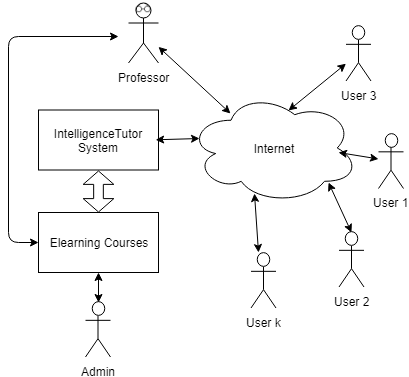
\includegraphics[width=0.6\textwidth]{Figures/se1.png}
	\caption{Intelligence Tutor System context}
	\label{ITSC}
\end{figure}
\section{Objectives}
According to the challenges of online group studying, we figure out that the most important problems are the problem \#1 which is the students with their antipathy of group study or teamwork. When we solve this problem, the rest issues can be fixed quickly and effectively. To do so, we propose a smart MediatorBot with three objectives such as: 
\begin{itemize}
	\item Generate hints to help users solve the topic or problem automatically
	\item    Identify the debated or clarify the problem
	\item Intervene in the conversation to clarify the problem: identify the opportunities for intervention, answer the related topic question of users
\end{itemize}
\begin{figure}
	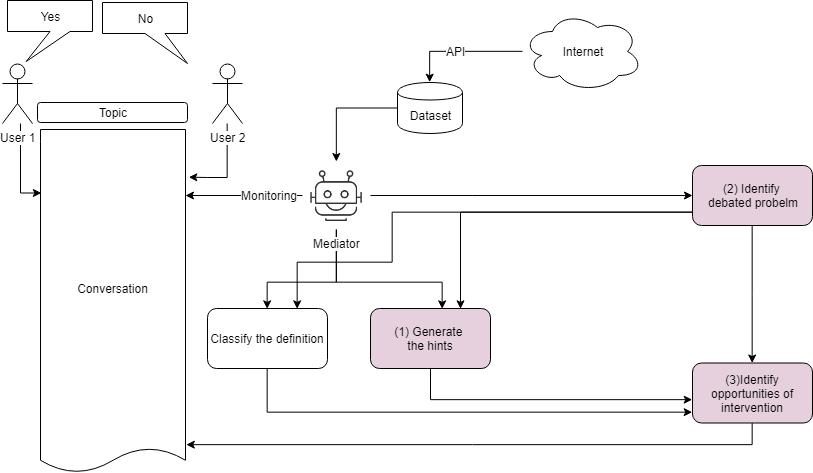
\includegraphics[width=0.7\textwidth]{Figures/2.png}
	\caption{Mediator system}
	\label{MS}
\end{figure}


\subsection{Generate the hints to help users solve the topic or problem automatically}
The hint generation module is very useful to teach students how to find the correct solution and building their knowledge step-by-step, including how to write an answer, what do they need to focus on, and how to express and understand a concept. A major benefit of the automatic hint generation is that it can be personalized for each student and fix their knowledge gaps. Moreover, it is also a useful exploration for the future task of automatic generation of the content of courses. Additionally, these generated hints are beneficial for teachers or instructor. Furthermore, they could select one hint and refine them, which makes the generated hints more student-friendly. Especially for the online group learning, the generated hints can help the student want to work more in the group without their antipathy which is the most major reason for many problems group work. First, this module should ensure the contextual relevance between questions, answers, and considered concepts. This involves task complex contextual information, such as definitions which generally contain many aspects (e.g., concepts, ideas, equations). Second, it requires generating diversified hints for each concept, which makes the task more challenging.

\subsection{Identify the debated problem}

According to the students' conversations based on the given topic or assignment, identify the debated problem makes more values for learning intelligence effort. Here we argue that depending on the type of question and its’ following conversation, students' sentiments, a new system of automatically identify the debated problem is proposed. This system will enable to clarify the problem of conversation quickly and keep students on the right track of conversation to follow the assignment or topic, at low-cost in many different educational domains. This approach provides more
detail result than the current practice of word cloud, while it is
faster than sentiment analysis approach.


\subsection{Intervene in the conversation to clarify the problem}
We propose developing a module, which interactively identifies the opportunities for intervention, answers the related topic question of students. An intelligent tutoring system with this module will solve the above-mentioned problems as follows:
\begin{itemize}
	\item Not only prevent the conflict problem but also encourage students to work together in the online group learning
	\item No need mentors if students need help, support
	\item Students can get multiple levels of hints, find their files, media, text, etc., to approach concepts or solve a given question, problems.
	\item     Monitoring of learning progress become easier because one can both automatically evaluate and measure the number of hints and quality of students’ answers and intervene in the right way the problems of group learning 
	\item     Interactively generating content from unstructured text, preventing the conflicts conversation and encouraging students learning automatically help the professors save a lot of time because they will be able to quickly review and modify the existing content to approach the best quality of training with low cost.
\end{itemize}


Hence, dealing with the problem of generating appropriate and effective learning content is our third objective.

\begin{comment}
\section{Table layout tests}

Tables have the same constraints than the figures, except for the caption that has to be on top.


\begin{table}
		\parbox{0.65\textwidth}{\caption{Test of a long table caption, with linebreak.}} % Contrainte manuelle de la largeur de la légende
		\begin{tabular}{|c|c|c|c|c|c|c|c|}
		\hline
			{\bf titre} & {\bf titre} & {\bf titre} & {\bf titre} & {\bf titre} & {\bf titre} & {\bf titre} & {\bf titre} \\
	  \hline
			blá & blá & blá & blá & blá & blá & blá & blá \\
	  \hline
			blá & blá & blá & blá & blá & blá & blá & blá \\
	  \hline
			blá & blá & blá & blá & blá & blá & blá & blá \\
	  \hline
			blá & blá & blá & blá & blá & blá & blá & blá \\
	  \hline
			blá & blá & blá & blá & blá & blá & blá & blá \\
	  \hline
			blá & blá & blá & blá & blá & blá & blá & blá \\
	  \hline
		\end{tabular}
\end{table}


\section{References test}

\subsection{References to the bibliography}

\subsection{References to the list of references "refs"}

References from the list of references "refs", declared at the beginning of the document \citerefs{Test}.

\subsection{References to a label of the document}

Reference to a Figure associated to a label: Figure \ref{fig:vueEts}.

\subsection{URL references}

\subsubsection{Test of "href"}

Href is used to integrate a link to a text:
\href{http://www.etsmtl.ca/Etudiants-actuels/Cycles-sup/Realisation-etudes/Guides-gabarits}{Link to the template page.}.

\subsubsection{Test de url}

Url is used to format a clickable link:
\url{http://www.etsmtl.ca/Etudiants-actuels/Cycles-sup/Realisation-etudes/Guides-gabarits}.
\end{comment}
%%- Third demo chapter -%%
\chapter{Research methodology}



This research tackles the problem of intervening students' conversation to encourage them to study and build their knowledge. The conversational ITS identifies the chance of intervention, gives hints to the student, and then analyzes their answer using machine learning algorithms during students' conversation. When the students' conversations based on the given topic have the signals of conflict which can be recognized by the emoticons, contradict description, it is classified as being a positive, negative, or unknown problem. The system must analyze the main reason for conflict, the opportunities for intervention,  and give an appropriate hint to help them answer the question, reconcile the conflict, and encourage the study or understand the topic, assignment. 
\begin{figure}
	\centering
	
	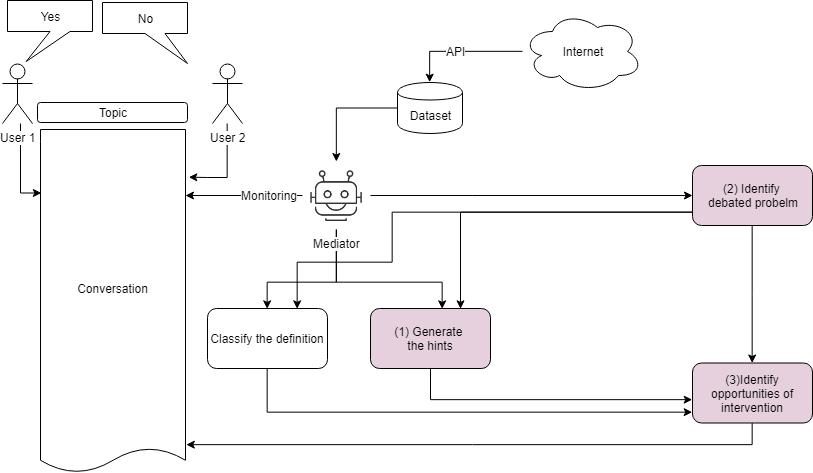
\includegraphics[width=0.75\textwidth]{Figures/2.png}
	
	\caption{MediatorBot System }
	\label{fig:autotutor}
\end{figure}
The system at Figure \ref{fig:autotutor} is powered by a database of questions, answers, hints, emoticons, concept descriptions. The component generating the hints is called the “hint generator” model. To this end, we propose a feedback and hint generation model capable of generating meaningful, personalized, pedagogical hints based on the right definitions of many concepts. Identify the debated problem and opportunity of intervention models are proposed to monitor, keep, and encourage students to study with their positive feeling.  In addition, we also investigate how the system may be capable of efficiently adapting its content and tutoring strategies to individual group students.



\section{Methodology for Sub-objective 1}
\begin{figure}
	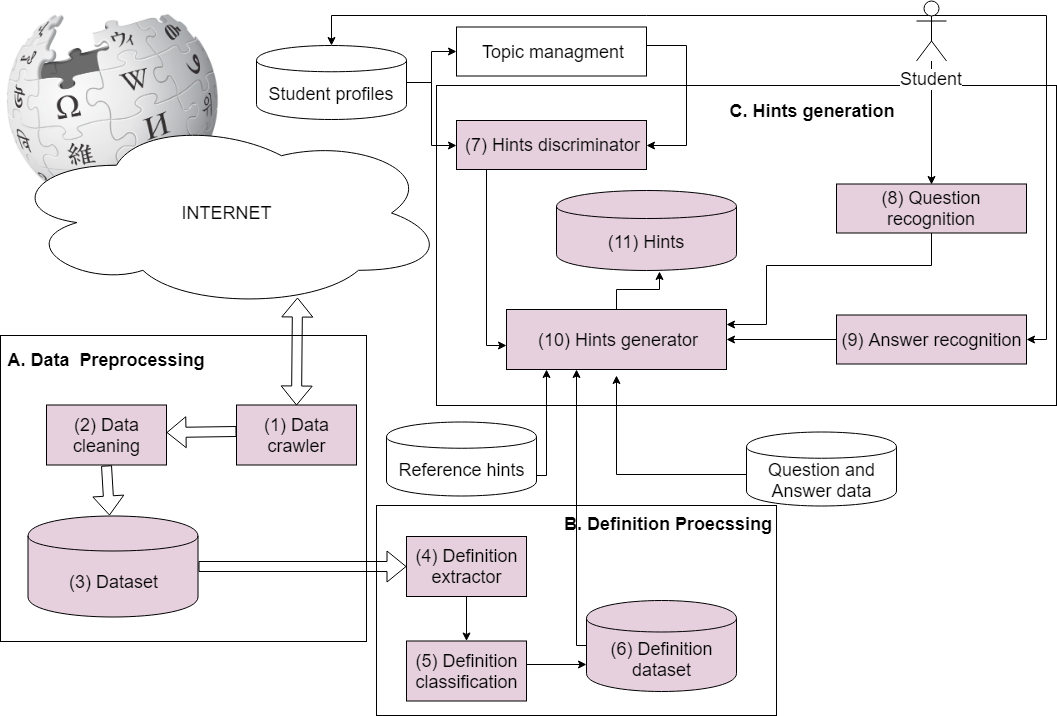
\includegraphics[width=0.7\textwidth]{Figures/23.png}
	\caption{Hints generator system}
	\label{hintst}
\end{figure} 


We propose a method to generate new hints which can be integrated into the Intelligent tutor system as the new advantage of value. The hint generator is presented in Figure \ref{hintst}, is built on three components: Data preprocessing, Definition processing, and Hints generation. We introduce an attention mechanism and relevance control mechanism to boost it.  

We crawl the text stream from unstructured data sources such as Wikipedia with a given domain--specific (e.g.,  Machine learning) which is presented in Figure \ref{datapred}. By using the wikipedia-api\footnote{https://pypi.org/project/wikipedia/} which is easy to access and parse data from Wikipedia, we extract the  list of relevance recursive subcategories according to the given domain--specific. 

\begin{figure}[h]
	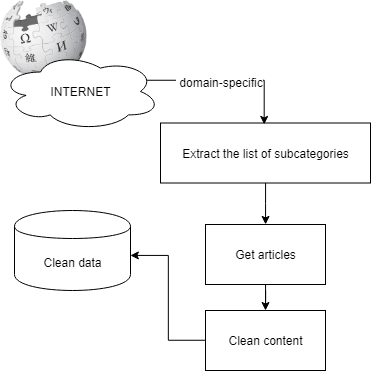
\includegraphics[width=0.4\textwidth]{Figures/cr.png}
	\caption{Data preprocessing}
	\label{datapred}
\end{figure} 

Based on the structure content list of wikipedia article\footnote{https://en.wikipedia.org/wiki/Main\_Page}, we extract the section "See also" by another recursive function to get more relevance keyword of this domain--specific. According to the list of relevance keywords, we crawl the articles, respectively. After cleaning all of the Unicode and converting all the mathematical expression to the standard string we save the clean--content to the clean-data which is used for definition extraction component. 

The component of definition extractor is presented in Figure \ref{defex}. Based on the clean data, we extract all the sentence tokens of articles and acronyms of technical keywords. According to the list of sentence tokens, we extract the subject of each sentence by using the Spacy API \footnote{https://spacy.io/api} which is the \textit{Doc} and the \textit{Vocab}. The \textit{Doc} object owns the sequence of tokens and all their annotations. The \textit{Vocab} object owns a set of look-up tables that make common information available across documents. On the other hand, the acronyms of technical keyword is extracted by using algorithm which proposed by Schwartz and Hearst \footnote{http://www.cnts.ua.ac.be}. After get the description of concept and the first sentence of relevance wikipedia article, we save them to the list of concept description.


\begin{figure}
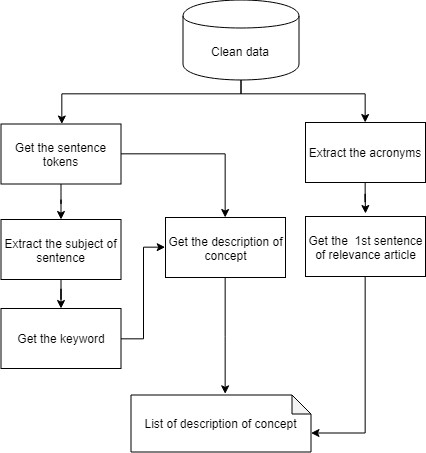
\includegraphics[width=0.45\textwidth]{Figures/df1.png}
\caption{Definition extractor}
\label{defex}
\end{figure} 

 
According to the extraction definition dataset, we observe that one concept may have one or many description, hence we compute the score for each descriptions by features as in Table \ref{tab:2}. We define that the first sentence of the wikiepdia article is the good definition and the rest is the not good definition. By using logistic classification algorithm, we train our model to classify the good and not good definition. Hower, we observe the oversampling scenario, so we increase the weight of good samples to approximately the not good ones. After classifying the definitions to good and not good definition  where good definition class is the class contained the exactly definitions, the other contained the explained definitions. 


\begin{table}[]
	\begin{tabular}{|l|l|lll}
		\cline{1-2}
		\textbf{Features}             & \textbf{Summary}              &  &  &  \\ \cline{1-2}
		\code{length\_of\_keyword}  & the number words in the keyword    &  &  &  \\ \cline{1-2}
		\code{length\_of\_description} & the number words in the description &  &  &  \\ \cline{1-2}
		\code{score\_keyword}          & inverse document frequency of keyword          & &  &  \\ \cline{1-2}
		\code{score\_description}          & inverse document frequency of concepts description          & &  &  \\ \cline{1-2}
		
		\code{ner\_in\_description}          & name of entity recognition within the description        & &  &  \\ \cline{1-2}
		
		
		\code{coreference\_in\_description}          & compute the coreference resolution score         & &  &  \\ \cline{1-2}
		
		\code{type\_of\_word}          & recognize type of word (verb, noun, etc.,)        & &  &  \\ \cline{1-2}
		
		\code{non\_of\_word}          & recognize the none of word (symbol, number, etc.,)        & &  &  \\ \cline{1-2}
		\code{pronouns\_rate}          &  the rate of $\frac{pronouns}{nouns}$  & &  &  \\ \cline{1-2}
		\code{keyword\_rate}          &  the rate of $\frac{keyword\_position}{length\_of\_description}$  & &  &  \\ \cline{1-2}
		\code{perplexity}          & the real value of perplexity of desciption  & &  &  \\\cline{1-2}
		\code{likelihood\_score}          & \begin{tabular}[c]{@{}l@{}}the log-likelihood probability score of description\\ based on sum of probability output by using language \\model\end{tabular} & &  &  \\ \cline{1-2}
	\end{tabular}
	\caption{Features of definition}
	\label{tab:2}
\end{table}
\begin{figure}
	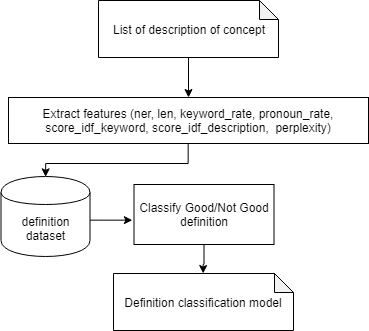
\includegraphics[width=0.5\textwidth]{Figures/dc1.png}
	\caption{Definition classification system}
	\label{datapre}
\end{figure} 
Given a conversation, we observe that users often use different types of questions as:
\begin{itemize}
	\item (a) definition
	\item (b) definition and explanation
	\item (c) two or more definitions contrasting each other
	\item (d) explanation
	\item (e) list of properties
\end{itemize}

These properties will be used in the future to evaluate if the student’s response is satisfactory. For example, with a question type (b) “definition and explanation” the system would expect to get some sort of a definition with accompanying explanation, and one of information only should not be considered as satisfactory. Hence, when the system identified the definitions are correct, it should explain more details or in another aspect of this issue.  For type (c) “contrast”,  the system should expect to get 2 contradict definitions. 

\begin{table}[]
	\begin{tabular}{|l|l|lll}
		\cline{1-2}
		\textbf{Features}             & \textbf{Summary}              &  &  &  \\ \cline{1-2}
		\code{length\_of\_hint}  & the number words in the hint     &  &  &  \\ \cline{1-2}
		\code{overlap\_question\_hint} & the rate of overlap between question and hint &  &  &  \\ \cline{1-2}
		\code{score\_keyterm}          & inverse document frequency of keyterm in hint          & &  &  \\ \cline{1-2}
		\code{keyhint\_keyquestion\_ratio}          & the ratio of $\frac{number\_of\_keyhint}{number\_of\_keyquestion}$     &  &  &  \\ \cline{1-2}
		\code{topic\_overlap}          & content overlap between the question and hint     &  &  &  \\ \cline{1-2}
		
		\code{pronouns\_rate}          &  the rate of $\frac{pronouns}{nouns}$ in hint  & &  &  \\ \cline{1-2}
		\code{keyword\_rate}          &  the rate of $\frac{keyword\_position}{length\_of\_hint}$  & &  &  \\ \cline{1-2}
		\code{perplexity}          & the real value of perplexity of hint  & &  &  \\ \cline{1-2}
		\code{ner\_in\_hint}          & name of entity recognition within the hint        & &  &  \\ \cline{1-2}
			\code{score\_of\_hint}          & \begin{tabular}[c]{@{}l@{}}the log-likelihood probability score of hints\\ based on sum of probability terms  by using language \\model based on RNN\end{tabular}       & &  &  \\\cline{1-2}
	\end{tabular}
	\caption{Features of hints}
	\label{tab:3}
\end{table}

Accordingly, the hints used for each type of the questions are different: e.g., the hints of type (b) encourage the students to address both of definition and explanation, and if one of them is missed, the system will explain more. The hints for type (c) should encourage contrasting the concepts.


The questions are recognized by keywords or  question structure:
\begin{itemize}
	\item  Recognize question words “what”, “is this/that” or the prompt word “define”
	\item Identified by the question words “what”, “is this/that” and the prompt “explain”
	\item Most reliably identified by the keywords “difference” or ”contrast” + “between”
	\item Explored the question words “why”, “how” or the prompt word “explain”    
\end{itemize}
Based on the reference of question and answer data, the features of hints are represented in Table \ref{tab:3}. On the other hand, the hints discriminator is considered based on the student answer and topic management to make the right hint for the learning student. The generator in Figure \ref{hints} uses an encoder-decoder LSTM framework. In order to ensure the contextual relevance with the hints, we propose the way of learning soft alignments between generated hints and news context and adaptively computes encoder-side context vectors. Moreover, it selects the amount of contextual information to predict the next word. In order to generate diversified hints, we use random sample strategy to generate hints with diverse topics. Our model is proposed based on a recurrent neural network (RNN). In the earlier of training, we use the maximum likelihood estimation (MLE) to pre-train the hint generator on training set until the generator reaches convergence. Afterward, MLE is utilized to pre-train hint classifier with real hints and auto hints generated by our generator. After the pre-training, the generator and classifier are trained alternatively until convergence. In order to evaluate our method, we use both automatic evaluation metrics to show that the generated new hints are close to human hints and manual annotations to evaluate their quality.  Our goal is to generate diversified hints for different topics and with various degrees of relevance by utilizing a random sample and a relevance control mechanism. 

\begin{figure}
	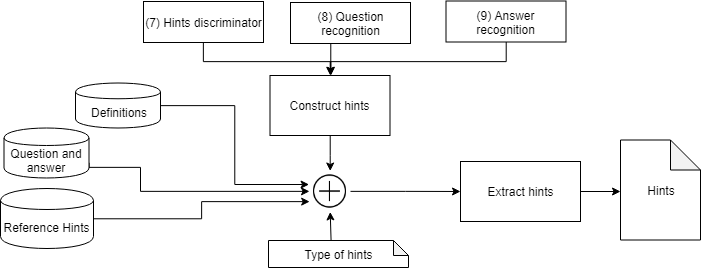
\includegraphics[width=.9\textwidth]{Figures/ht2.png}
	\caption{Hints generator component system}
	\label{hints}
\end{figure} 


\section{Methodology for Sub-objective 2}
We next present a brief overview of the system identified the debated problem system based on the conversation of students which is illustrated in Figure \ref{dpr}
\begin{figure}
	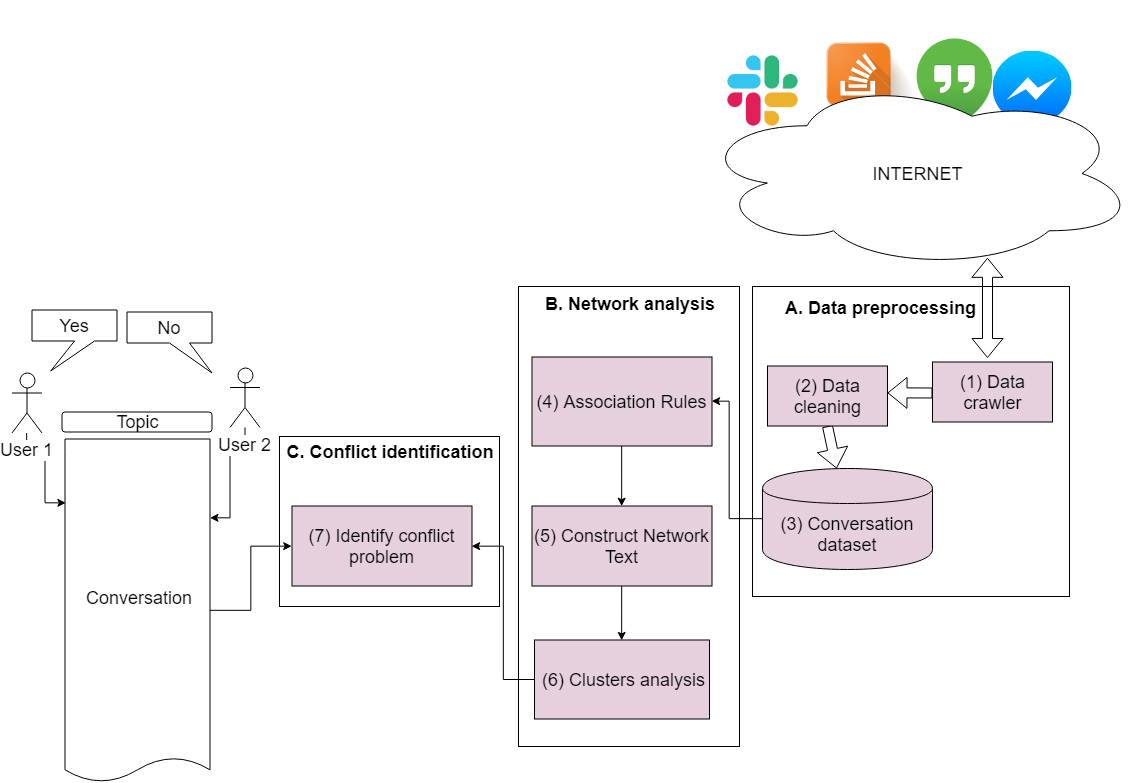
\includegraphics[width=0.9\textwidth]{Figures/32.png}
	\caption{Identify debated problem }
	\label{dpr}
\end{figure}

In this system, the conversations of a specific-domain (e.g., deep learning) are crawled from slack, StackOverflow, hangout, messenger via their application protocol interfaces (APIs). After we get a large volume of conversations, we conduct pre-process, which clean all the Unicode types (e.g., Chinese, Japanese) or any symbol and delete irrelevant conversations to the topic which we investigate at Figure \ref{dataobj2}


\begin{figure}
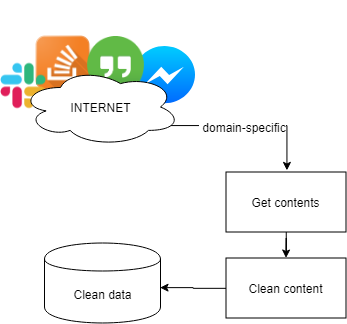
\includegraphics[width=0.4\textwidth]{Figures/dts.png}
\caption{Identify debated problem}
\label{dataobj2}
\end{figure}


The dominant words are found by using a word cloud applications. We remove unsuitable dominant words to opinion words, this includes removing conjunction, pronoun, numbers, date,  URL links, and others. After that, the association rules between dominant words are calculated.  They find the interesting association and/or correlation relationship among a large set of data items and show attribute value conditions that occur frequently in the conversation dataset. We construct the network text of dominant words, which include weight edge result for association rules process. Then, we analyze the data by creating context, keyword, and sense from network text. In network analysis, we employ centrality the most important words in the networks. Hence by analyzing the students' conversations,  we identify the debated problem and recognize the clarify problem scales. 




\section{Methodology for Sub-objective 3}

\begin{figure}
	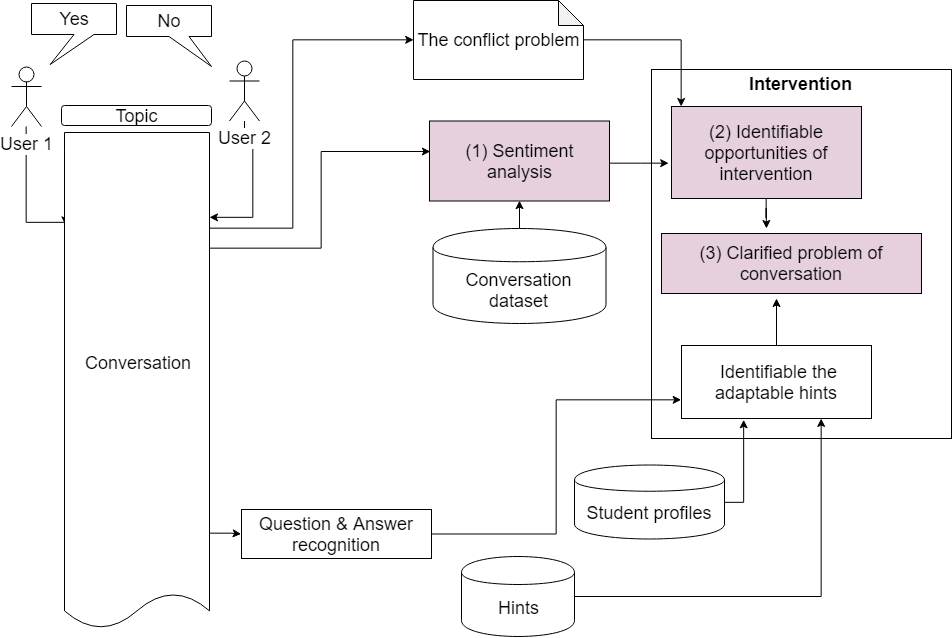
\includegraphics[width=0.7\textwidth]{Figures/58.png}
	\caption{Intervention system}
	\label{intervention}
\end{figure}
Figure \ref{intervention} illustrates the architecture of the third system, which interactively identifies the opportunities for intervention and helps students solve their problems during conversations. The input data is a collection of various different materials such as hints, clarify a problem, sentiment analysis, questions and answers, students' questions and answers recognition.  We extract the fact of sentiment words included emoticons from the students' conversations, then match all the emoticon symbols to its' meaning. After that, we analysis the sentimental of each student according to their conversation. Based on the clarify problem scales and sentimental analysis, the opportunity of intervention is identified by using the hidden Markov chain algorithm. Each state of sentiments is processed by the Sentiment Analysis which is recorded as an input recommendation system. In order to automatically help and encourage students to study, a system for processing a variety of data related to the topic and language is proposed based on Natural Langauge Processing (NLP) technology.  By considering these questions and answers respected with the students’ answers and their profile, the relevance and adapter hints are generated. The scoring and confidence model is finally applied to evaluate the quality of the output data.  Sentiment  analysis also  is aware of conversation mining which needs to be analyzed,  processed, reasoned and induced texts with emotional labels. It extracts polarity and subjectively from the semantic orientation which refers to the strength of words and polarity text or phases. We approach the to machine learning method where sentiment detection is labeled as emoticons.  Emoticon and Contratict term classification is the core problem of sentiment analysis technology, is to judge tendency in the  review, then is considered as the weight of the relevance term. According to the limited data information, we use Support Vector Machine (SVM) \cite{Saif} to find the best compromise between the complexity and the learning ability, in order to get the best generalization ability up to 80\% of accuracy on the test set. The feature vector is created as the table \ref{tab:svm}

\begin{figure}
	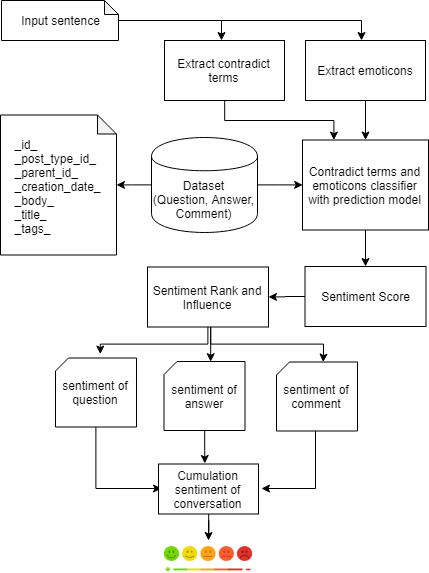
\includegraphics[width=0.6\textwidth]{Figures/st5.png}
	\caption{Sentiment analysis}
	\label{sentiment}
\end{figure}
\begin{table}[]
	\begin{tabular}{|l|l|lll}
		\cline{1-2}
		\textbf{Features}             & \textbf{Summary}              &  &  &  \\ \cline{1-2}
		\code{number\_of\_positive\_word}  & the number positive words  &  &  &  \\ \cline{1-2}
		\code{number\_of\_negative\_word}  & the number negative words  &  &  &  \\ \cline{1-2}
		\code{tag\_of\_emoticons}  & the tag of emoticons  &  &  &  \\ \cline{1-2}
		\code{scale\_of\_sentiment\_adjective}  & the scale score of sentiment adjective  &  &  &  \\ \cline{1-2}
		\code{frequency\_of\_sentiment\_adjective}  & the frequency  of sentiment adjective  &  &  &  \\ \cline{1-2}
	\end{tabular}
	\caption{Table features of sentiment analysis}
	\label{tab:svm}
\end{table}
On the other hand, Convolution neural networks (CNN) is good at learning the characteristics of the invariance, and SVM can find the optimal classification surface for the characteristics. In our methodology, we combine both SVM and CNN to solve text analysis. Because the output vectors of the pooling layer of CNN are represented by distributed features of input samples, the distributed feature representation can be used as feature input in SVM. Therefore, CNN is utilized as an automatic feature investigator, then SVM is used as an emoticon classifier, and both of them are combined to deal with sentiment analysis to generate the weight (label) of each student. \cite{Kim} applied the idea of CNN to text classification, and implemented a CNN-based text classification model for classifying sentences. show that CNN-based text classification method is more accurate than the best at that time.  Moreover, the using of word order for text categorization with convolutional neural network is proposed in \cite{Johnson}. 

\begin{figure}
	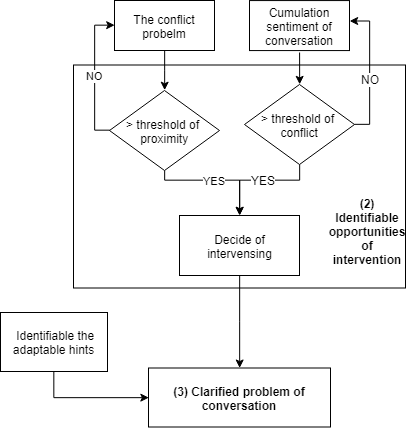
\includegraphics[width=0.5\textwidth]{Figures/tsv.png}
	\caption{Intervention decision}
	\label{decide}
\end{figure}
In addition to the text classification model based on CNN, as shown in Figure \ref{sentiment}, is the input layer, the convolution layer, the pool layer, and the output layer. Figure \ref{sentiment} text emotion classification model based on CNN The last layer of text sentiment based on CNN is the full connection layer. The input of this layer is the feature vector outputted from the pool layer, and the output of each category label classified according to the probability size. However, SVM the theory of  VC theory and the minimum structural risk. So SVM represents the data feature vectors in the feature space, classified hyperplane.  For linear,  SVM can map space through a kernel function, and then transform the linear non-separable problem into a separable problem.  That is,  CNN the characteristics of the invariance and SVM can find the optimal classification surface for the characteristics based on the given emoticon dictionary\footnote{https://emojipedia.org}. Hence, the opportunity for intervention is identified based on the serious of conversation and the debated problem. To give the right intervention, the system analysis students' questions and answers including the adaptable hints. In the question and answer analysis, we focus on analyzing and quantifying the relation with question and answer. We use bidirectional LSTM model to measure the relevance between them. Then, we use a feed-forward network with shared parameters to learn the relevance between question and answer. The output is a relevance score between question and answer, so it is the particular feature of identifying the adaptable hints. 


\begin{comment}

\chapter{Experimentation and Results}
\section{Environment experiment}
\subsection{Initial environment experiment}
The Messenger Platform provides a set of REST APIs that give  the tools to create awesome Messenger experiences. From sending rich messages, to finding your existing customers on Messenger, to customizing your bot and more, our APIs are the primary way you will work with the Messenger Platform. Hence, our environment experiment is setup as the Figure \ref{env}.
\begin{figure}
	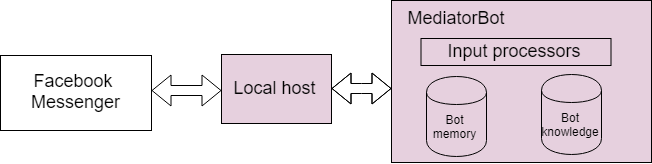
\includegraphics[width=0.6\textwidth]{Figures/ue1.png}
	\caption{Environment experiment}
	\label{env}
\end{figure}

\section{Result}
\end{comment}

%%%%%%%%%%%%%%%%%%%%%%%%%%%%%%%%%%%%%%%%%%%%%%%%%%%
% BIBLIOGRAPHY AND REFERENCES
%%%%%%%%%%%%%%%%%%%%%%%%%%%%%%%%%%%%%%%%%%%%%%%%%%%



%%- Bibliography -%%

% Single spacing for the bibliography
\begin{thebibliography}{01}
	\bibitem{Brown}  Brown, J. S., \& Burton, R. R. (1975). Multiple representations of knowledge for tutorial reasoning. In D. G. Bobrow \& A. Collins (Eds.), inmal-n ,rd ,zaitng (pp. 311--349). New York: Academic Press.
		\bibitem{Tchounikine}  Tchounikine P. (2002) Quelques éléments sur la conception et l'ingénierie des EIAH, In 2ème assises nationales su GDR I3, pp 233-246. Nancy, France.
	
\bibitem{Woolf2009}Woolf, BP (2009). Building intelligent interactive tutors. Burlington: Morgan
Kaufmann Publishers
		\bibitem{Sottilare}	Sottilare, R, Graesser, AC, Hu, X, Goldberg, B (Eds.) (2014). Design recommendations
	for intelligent tutoring systems: instructional management, (vol. 2). Orlando:
	Army Research Laboratory
	\bibitem{VanLehn2006}VanLehn, K. (2006). The behavior of tutoring systems. International Journal of
	Artificial Intelligence in Education
	, 16, 227
	–265.	
\bibitem{Aleven2009}	Aleven, V, Mclaren, BM, Sewall, J, Koedinger, KR. (2009). A new paradigm for
	intelligent tutoring systems: example-tracing tutors. International Journal of
	Artificial Intelligence in Education, 19(2), 105–154
	
	
\bibitem{Koedinger1997}		Koedinger, KR, Anderson, JR, Hadley, WH, Mark, M. (1997). Intelligent tutoring
	goes to school in the big city. International Journal of Artificial Intelligence in
	Education, 8, 30–43.
	
	
	
\bibitem{Ritter2007}		Ritter, S, Anderson, JR, Koedinger, KR, Corbett, A. (2007). Cognitive tutor: applied
	research in mathematics education. Psychonomic Bulletin \& Review, 14, 249–255.
	Rochelle, J, Feng, M, Murphy, R, Mason, C. (2016). Online mathematics homework
	
\bibitem{Falmagne2013}	Falmagne, J, Albert, D, Doble, C, Eppstein, D, Hu, X (2013). Knowledge spaces:
	applications in education. Berlin-Heidelberg: Springer	
		
		
\bibitem{Sabo2013}		Sabo, KE, Atkinson, RK, Barrus, AL, Joseph, SS, Perez, RS. (2013). Searching for the
		two sigma advantage: evaluating algebra intelligent tutors. Computers in
		Human Behavior, 29(4), 1833–1840.
		\bibitem{Lesgold1992}	Lesgold, A, Lajoie, SP, Bunzo, M, Eggan, G (1992). SHERLOCK: a coached practice
		environment for an electronics trouble-shooting job. In JH Larkin, RW Chabay
		(Eds.), Computer assisted instruction and intelligent tutoring systems: shared
		goals and complementary approaches, (pp. 201–238). Hillsdale: Erlbaum.
		
		
		
		
\bibitem{Dzikovska2014}		Dzikovska, M, Steinhauser, N, Farrow, E, Moore, J, Campbell, G. (2014). BEETLE II:
		deep natural language understanding and automatic feedback generation
		for intelligent tutoring in basic electricity and electronics. International
		Journal of Artificial Intelligence in Education, 24, 284–332.
		
\bibitem{Fletcher2012}	Fletcher, JD, \& Morrison, JE (2012). DARPA Digital Tutor: assessment data (IDA
Document D-4686). Alexandria: Institute for Defense Analyses.		
		
		
		
\bibitem{Mitrovic2007}		Mitrovic, A, Martin, B, Suraweera, P. (2007). Intelligent tutors for all: the constraintbased approach. IEEE Intelligent Systems, 22, 38–45.
\bibitem{VanLehn2011}		VanLehn, K. (2011). The relative effectiveness of human tutoring, intelligent tutoring
		systems and other tutoring systems. Educational Psychologist, 46, 197
		–221.
\bibitem{Johnson2016}	Johnson, WL, \& Lester, JC. (2016). Face-to-face interaction with pedagogical
	agents, twenty years later. International Journal of Artificial Intelligence in
	Education, 26(1), 25–36.	
		
\bibitem{Graesser2016}	Graesser, AC. (2016). Conversations with AutoTutor help students learn.
	International Journal of Artificial Intelligence in Education, 26, 124–132	
		
	\bibitem{Nye2014a}	Nye, BD, Graesser, AC, Hu, X. (2014a). AutoTutor and family: a review of 17 years
		of natural language tutoring. International Journal of Artificial Intelligence in
		Education, 24(4), 427–469.
	\bibitem{Nye2014b}	Nye, BD, Graesser, AC, Hu, X. (2014b). AutoTutor in the cloud: a service-oriented
		paradigm for an interoperable natural-language ITS. Journal of Advanced
		Distributed Learning Technology, 2(6), 35–48
		
		
		
		
		\bibitem{Atkinson2002}	Atkinson, RK. (2002). Optimizing learning from examples using animated
		pedagogical agents. Journal of Educational Psychology, 94, 416.
		
			\bibitem{Craig2002}	Craig, SD, Gholson, B, Driscoll, D. (2002). Animated pedagogical agents in
		multimedia educational environments: effects of agent properties, picture
		features and redundancy. Journal of Educational Psychology, 94, 428.
		
		
		\bibitem{Johnson2000}	Johnson, WL, Rickel, JW, Lester, JC. (2000). Animated pedagogical agents: face-toface interaction in interactive learning environments. International Journal of
		Artificial Intelligence in Education, 11(1), 47–78.
		
			\bibitem{McNara2010}Graesser, A, \& McNamara, D. (2010). Self-regulated learning in learning
		environments with pedagogical agents that interact in natural language.
		Educational Psychologist, 45(4), 234–244.
		\bibitem{Moreno2001}Moreno, R, Mayer, RE, Spires, HA, Lester, JC. (2001). The case for social agency in
		computer-based teaching: do students learn more deeply when they
		interact with animated pedagogical agents? Cognition and Instruction, 19(2),
		177–213.
		
			\bibitem{Craig2015}Craig, SD, Twyford, J, Irigoyen, N, Zipp, SA. (2015). A test of spatial contiguity for
		virtual human’s gestures in multimedia learning environments. Journal of
		Educational Computing Research, 53(1), 3–14.
		
		
	\bibitem{Graesser2014}	Graesser, AC, Li, H, Forsyth, C. (2014). Learning by communicating in natural
		language with conversational agents. Current Directions in Psychological
		Science, 23, 374–380.
		

		\bibitem{Kim2007}	Kim, Y, Baylor, AL, Shen, E. (2007). Pedagogical agents as learning companions:
		the impact of agent emotion and gender. Journal of Computer Assisted
		Learning, 23(3), 220–234
	\bibitem{Johnson2000}Johnson, WL, Rickel, JW, Lester, JC. (2000). Animated pedagogical agents: face-toface interaction in interactive learning environments. International Journal of
	Artificial Intelligence in Education, 11(1), 47–78.	
		
		\bibitem{Kim2016}	Kim, Y, \& Baylor, AL. (2016). Research-based design of pedagogical agent roles: a
		review, progress, and recommendations. In
		
		
				\bibitem{Baylor2005}Baylor, AL, \& Kim, Y. (2005). Simulating instructional roles through pedagogical
		agents. International Journal of Artificial Intelligence in Education, 15(2), 95–115.
		
		
			\bibitem{Chan1990}	Chan, TW, \& Baskin, AB (1990). Learning companion systems. In C Frasson, G
		Gauthier (Eds.), Intelligent tutoring systems: at the crossroads of artificial
		intelligence and education, chapter 1. New Jersey: Ablex Publishing Corporation.
	
	
	%%%%%%%%%%%%%%	
		\bibitem{Freedman}  Freedman, R. (1999). Atlas: A plan manager for mixed-initiative, multimodal dialogue. AAAI ’99 Workshop on Mixed-Initiative Intelligence, Orlando.
	
		
			\bibitem{Nkambou}   R. Nkambou, J. Bourdeau \& R. Mizoguchi (2010). Advances in Intelligent Tutoring Systems. Springer. ISBN: 978-3-642-14362-5
		\bibitem{Bowen}   Bowen, W. G., Chingos, M. M., Lack, K. A., \& Nygren, T. I. (2014). Interactive learning online at public universities: Evidence from a six-campus randomized trial. Journal of Policy Analysis and Management, 33(1), 94-–111.	
		\bibitem{Pane}  Pane, J. F., Griffin, B., McCaffrey, D. F., and Karam, R. (2014). Effectiveness of cognitive tutor algebraI at scale. Educ. Eval. Pol. Anal. 36, 127–144. doi: 10.3102/0162373713507480
		\bibitem{Nesbit}  Nesbit, J. C., Adesope, O. O., Liu, Q., \& Ma, W. (2014). How Effective are Intelligent Tutoring Systems in Computer Science Education? Paper presented at the IEEE 14th International Conference on Advanced Learning Technologies (ICALT), Athens, Greece.
		\bibitem{Koedinger}  Koedinger K, Cunningham K, Skogsholm A, LeberB. An open repository and analysis tools for finegrained,longitudinal learner data. In: First InternationalConference on Educational Data Mining. Montreal, Canada; 2008, 157–166
		\bibitem{Boulay}  Du Boulay, B. (2016) Artificial Intelligence as an Effective Classroom Assistant. IEEE Intelligent Systems, 31(6), pp. 76-81. APA handbook of Educational Psychology. Washington, DC: Amercian Psychological Association
		\bibitem{Lane}  K. L. Lane, H. M. Menzies, R. P. Ennis, and J. Bezdek, School-wide Systems to Promote Positive Behaviors and Facilitate Instruction, Journal of Curriculum and Instruction (JoCI) Copyright 2013 June 2013, Vol. 7, No. 1, Pp. 6--31 ISSN: 1937-3929 http://www.joci.ecu.edu doi:10.3776/joci.2013.v7n1p6-31
		\bibitem{Graesser}  Graesser, A. C., Wiemer-Hastings, P., Wiemer-Hastings, K., Har- AUTOTUTOR 191 ter, D., Person, N. K., \& the Tutoring Research Group (2000). Using latent semantic analysis to evaluate the contributions of students in AutoTutor. Interactive Learning Environments, 8, 129--148.
		\bibitem{Hume}  Hume, G. D., Michael, J. A., Rovick, A., \& Evens, M. W. (1996). Hinting as a tactic in one-on-one tutoring. Journal of the Learning Sciences, 5, 23--47.
		\bibitem{Wiemer}  Graesser, A. C., Wiemer-Hastings, K., Wiemer-Hastings, P., Kreuz, R.,\& the Tutoring Research Group (1999). AutoTutor: A simulation of a human tutor. Journal of Cognitive Systems Research, 1, 35--51.
		\bibitem{Tsovaltzi}  D. Tsovaltzi et al. A Multi-Dimensional Taxonomy for Automating Hinting. In Intelligent Tutoring Systems  - 6th International Conference, ITS 2004, LNCS. Springer, 2004. 
	
		
		
		
\bibitem{Abhang}L. B. Abhang  and M. Hameedullah. Determination of optimum parameters for multi-performance characteristics in turning by using grey relational analysis, in International Journal of Advanced Manufacturing Technology, 2012



\bibitem{Kumar} R. Kumar, H. Ai, J. L. Beuth, and C. P. Rose, “Socially Capable Conversational Tutors can be effective in Collaborative Learning Situations”, Intelligent Tutoring System, 2010, 156--164
\bibitem{Tegos} Tegos,  S.,  \&  Demetriadis,  S.  (2017). Conversational  Agents  Improve Peer  Learning  through  Building  on Prior  Knowledge.Educational Technology \& Society, 20(1), 99–111


\bibitem{Adamson} Adamson, I. Howley and C. P. Rosé, "Enhancing Scientific Reasoning and Discussion with Conversational Agents," in IEEE Transactions on Learning Technologies, vol. 6, no. 3, pp. 240-247, July-Sept. 2013.



\bibitem{David M}David M. Blei and John D. Lafferty. 2005. Correlated topic models. In Proceedings of the 18th International Conference on Neural Information Processing Systems (NIPS'05), Y. Weiss, B. Schölkopf, and J. C. Platt (Eds.). MIT Press, Cambridge, MA, USA, 147-154.

\bibitem{Lipponena}Lipponen, L. (2002). Exploring foundations for computer-supported collaborative learning. In G. Stahl (Ed.),
Proceedings of the Computer-supported Collaborative Learning 2002 Conference, Hillsdale, NJ: Erlbaum, 72--81.

	\bibitem{Lipponenb}Lipponen, L., Rahikainen, M., Hakkarainen, K., \& Palonen, T. (2002). Effective participation and discourse through
a computer network: Investigating elementary students' computer-supported interaction. Journal of Educational
Computing Research, 27, 353--382. 
\bibitem{Johnson}Johnson, D.W., \& Johnson, R.T. (1987). Creative conflict, Edina, MN: Interaction Book Company. 
\bibitem{Kagan}Kagan, S. (1998). Teams of four are magic! Cooperative Learning and College Teaching, 9 (1), 9. 
\bibitem{Bean}Bean, J. C. (1996). The professor’s guide to integrating writing, critical thinking, and active learning in the
classroom, San Francisco: Jossey-Bass. 

\bibitem{Kim} Kim Y. Convolutional neural networks for sentence classification [C]//
Proceedings of the 2014 Conference on Empirical Methods in Natural
Language Processing. 2014: 1746-1751.
\bibitem{Johnson} Johnson R, Zhang T. Effective use of word order for text categorization
with convolutional neural networks [DB/OL]. 


\bibitem{Kerr}Kerr, N.L., \& Bruun, S.E. (1983). Dispensability of member effort and group motivation losses: free rider effects.
Journal of Personality and Social Psychology, 44, 78-94. 
\bibitem{Hara}Hara, N., \& Kling, R. (2000). Students' distress with a web-based distance education course. Information,
Communication and Society, 3 (4), 557-579. 


\bibitem{Myung} Koh, Myung-Hwa \& Hill, Janette. (2009). Student perceptions of group work in an online course: Benefits and challenges. Journal of Distance Education. 23. 69-92. 

\bibitem{Saif}H. Saif, Y. He and H. Alani, “Alleviating Data Scarcity for Twitter
Sentiment Analysis”. Association for Computational Linguistics, 2012
\end{thebibliography}
\begin{comment}
%%- Other list of references, "refs" example --%
%%%%%%%%%%%%%%%%%%%%%%%%%%%%%%%%%%%%%%%%%%%%%%%%%%%
% IMPORTANT: HOW TO COMPILE AND PRINT ADDITIONAL REFERENCES (replace "refs" by the chosen name)
%%%%%%%%%%%%%%%%%%%%%%%%%%%%%%%%%%%%%%%%%%%%%%%%%%%
% Follow these three steps:
%   1. Compile the document once, to save the used references in refs.aux
%   2. Compile the references
% 		- On Linux: Use the "bibtex refs" command in the document folder
%		- On MacOSX (MacTex distribution): Use the "/usr/texbin/bibtex refs" command in the document folder
%		- On Windows: Edit the "update_refs.bat" script to put the right suffix ("refs" here), and launch the script
%   3. Recompile the document TWICE
%%%%%%%%%%%%%%%%%%%%%%%%%%%%%%%%%%%%%%%%%%%%%%%%%%%

\newpage
% Same commands than for the bibliography, only with the "refs" suffix
\begin{spacing}{1}
	%\nociterefs{*}
	\bibliographystylerefs{bibETS}
	\addcontentsline{toc}{chapter}{LIST OF REFERENCES}

	\bibliographyrefs{refs}

\end{spacing}
\end{comment}
\begin{appendices}
	\chapter{Implementation and Results}


In this experiment we had undergraduate and graduate students from McGill University (COMP-551) try to use our system (Korbit). The experiment was carried out in-class. We instroduced the system to students for frist 5 minutes which was followed the demo video, then highlighted how to write natural language answers and the concept tree building auxiliary task. After that, the students spent 30-40 minutes trying out the system for their studying. Students gave us the feedback after finishing their work. The experiment was conducted on the evenings of February 6th and February 8th, 2019. To solve disengaged students, students with less than 05 user utterances are excluded from this analysis. We also excluded 4 other students who were clearly abusing or playing around with the system instead of following the exercises given. There are four evaluated components in this experiment:\\
1) Automatically generated hints \\ 
2) New student model \\ 
3) Concept tree visualization \\
4) Concept tree building \\
5) Selection task.\\
We evaluated three variants of our system\footnote{Source: Ai-educate}:
%\begin{itemize}
%	\item (Handicapped) System, where the student model is not utilized at all
%	\item (Handicapped) System, where the student model is not utilized by the policy for selecting next tutor engine states
%	\item (Full) Regular system, where the system uses all its modules including the student model.
%\end{itemize}
 \begin{table}[]
		\begin{tabular}{|l|l|l|}
			\hline
			& \begin{tabular}[c]{@{}l@{}}Human-Generated\\  Hints\end{tabular} & \begin{tabular}[c]{@{}l@{}}Machine-Generated \\ Hints\end{tabular} \\ \hline
			Sessions (Users)                                                                                                                                                    & {\color[HTML]{333333} 36}                                        & {\color[HTML]{333333} 36}                                          \\ \hline
			\begin{tabular}[c]{@{}l@{}}Number of times text-based hint \\ was shown (including the times it\\  was shown after the user clicked \\ “I don’t know”)\end{tabular} & 30 (100\%)                                                       & 19 (100\%)                                                         \\ \hline
			\begin{tabular}[c]{@{}l@{}}Number of times users improved \\ their next solution attempt after \\ hint was shown\end{tabular}                                       & 8 (26.67\%)                                                      & 8 (42.11\%)                                                       \\ \hline
			\begin{tabular}[c]{@{}l@{}}Number of times users gave a \\ “CORRECT” next solution attempt \\ after hint was shown\end{tabular}                                     & 5 (16.67\%)                                                      & 6 (31.58\%)                                                        \\ \hline

		\end{tabular}
				\caption{The experiment of generated hints}
\end{table}
The text-based hints generated by humans or by a machine automatically perform reasonably well. In previous experiments, we found that human-generated hints helped users to improve their answer by on average 10-30\% points (i.e. the probability of being “CORRECT” after a hint increased by 10-30\% points). The table above suggests that the hints in this experiment help improve the student answers 20\% - 50\% of the time and that 10\% - 30\% of the time the student’s next solution attempt is “CORRECT”.  When comparing the human-generated hints to the machine-generated hints, the table above shows that the machine-generated hints perform better. This may be an artefact of the fact that the machine-generated hints are created based on the reference solutions and therefore may reveal more information to the students. These numbers should therefore be interpreted with a grain of salt. If we stay on the conservative side, we may conclude that the machine-generated hints are overall comparable to the human-generated hints. This is still good news, because it means that we can automate one of the most important parts of the content creation pipeline.
	\chapter {Plan of researching}

\begin{figure}
	
	
		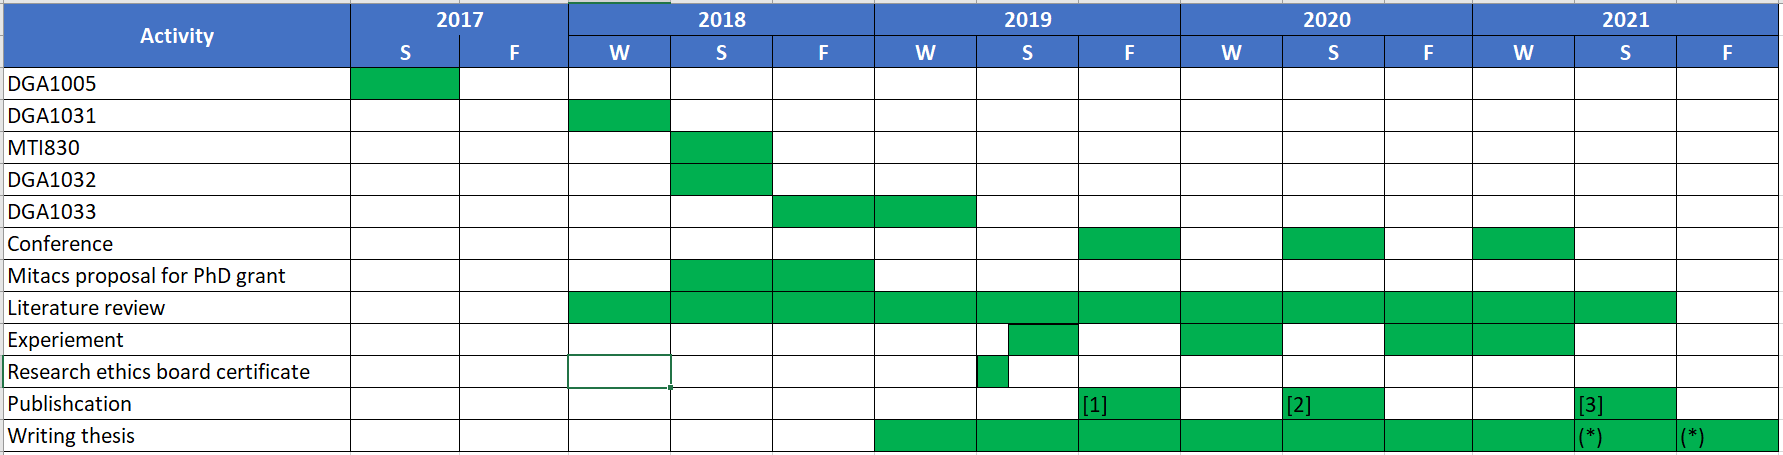
\includegraphics[width=\textwidth]{Figures/plan2.png}
	
	\caption{Work schedule}
\end{figure}

		\textbf{Journals:}
		\par [1] Journal of Artificial Intelligence Research 
		\par [2] Technology, Knowledge and Learning
		\par [3] Education and Information Technologies
		

		\textbf{Finished courses:}
		\par (1) DGA1005
		\par (2) MTI830
		



	\chapter{Evaluation Question Bank}
     \includepdf{"4"}
 \includepdf{"1"}
  \includepdf{"2"}
   \includepdf{"3"}

     \includepdf{"5"}
     


     
\end{appendices}

\end{document}
